\documentclass{article}
\usepackage{amssymb, amsfonts, amsmath, geometry, verbatim}
\geometry{letterpaper}
\usepackage[parfill]{parskip}    		% Activate to begin paragraphs with an empty line rather than an indent
\usepackage{graphicx}
\graphicspath{{./}}
\usepackage[nottoc]{tocbibind}
\newcommand{\R}{\mathbb{R}}

\title{Calculating the Solvent Exposed Surface Area of Proteins with Intersecting Spheres} % Feel free to change
\author{Gargi Kher, Neil Gupta}
\date{\today}

						
\begin{document}

\maketitle
\tableofcontents
\newpage
\section{Abstract}
Calculating the solvent-exposed surface area (SASA) of large biomolecules is an important problem in structural biology, especially in the case of proteins, where small changes in the molecule's shape can greatly limit the protein's ability to do its job. The fraction of a polar atom's surface area that is exposed to the engulfing solvent can be the difference between a stable hydrogen bond being formed with the solvent and a polar atom buried within the protein, which could prevent the protein from folding into its proper shape. Molecular dynamics simulations, which use computers to predict the time evolution of a molecular system also rely on accurate SASA calculations as a way to compute the enthalpy of hydration for the molecules in the system. Today, SASA is usually calculated based on an implicit solvation model, where the solvent is taken to be a continuous field that the molecules of interest sit in. The atoms are taken to be spheres of definite radius, and thus calculating the SASA of an atom involves calculating the fraction of the sphere that is exposed. The SASA of the entire molecule can be found by summing this quantity over all atoms. This paper gives a overview of \textsc{alphamol}, a way of analytically calculating the derivative of SASA with respect to time, a quantity which can be numerically integrated as part of a molecular dynamics simulation to predict the future state of a molecular system. We also discuss a previous way of computing SASA that \textsc{alphamol} improves upon. Finally we do some calculations of our own to benchmark the performance of these two methods and provide some modern context for where SASA computations are used.

\section{Previous Work}
Accurately and quickly calculating the SASA of proteins has been a problem that people have been trying to solve since the 1980's. One reason for this is the fact that the effective potential for solvation can be written $W=W_{elec}+W_{np}$, where $W_{elec}$ represents the electrostatic contribution and $W_{np}$ represents the nonpolar contribution to this potential. The second term depends heavily on the SASA value of the polar atoms in the molecule, as polar atoms with a low SASA value (buried polars) should to make hydrogen bonds to preserve the protein's structure. One of the earliest ways of computing this value was by Richmond (1984). His method involved modeling atoms as spheres and computing SASA as an application of the Gauss-Bonnet Theorem. This method was the basis for many future SASA calculators that optimized for attributes like speed or numerical stability. Other methods didn't focus as much on exact values in the interest of speed. The Shrake-Rupley algorithm (optimized by Legrand and Merz as discussed below), breaks up the spherical surface of each atom into a set of dots, and uses the fraction of dots that are exposed as a proxy for the exposed surface area. This is the default SASA calculator in Rosetta, a software package developed at the UW that allows for the computational analysis and design of protein structures. 
\subsection{Geometrical Representation of Atoms}
While atoms are comprised of protons, neutrons, and electrons, electrons are what give them their properties. Electrons make up the volume of an atom, and are more likely to be found closer to the nucleus than away. Because we don’t know for certain where electrons are in an atom, they can be represented by orbitals, or positions that give the probability of electrons being there. Orbitals can take on different shapes, generally resembling some type of dumbbell, but when these orbitals come together, they form a roughly spherical shape. This is why atoms are often modeled as spherical objects. (citation)
\subsection{Shrake-Rupley Algorithm}
The Shrake-Rupley Algorithm (Shrake and Rupley, 1973) is the standard way of calculating SASA by approximating the surface as a discrete set of voxels instead of a continuous surface. This can lead to inaccuracies, but the gains in speed are usually worth it. Prior exact algorithms could also fail if the protein surface was not continuous (i.e. an internal cavity is present) or the atomic radii are too small. This algorithm, once optimized by Legrand and Merz (1993) became a standard SASA calculator. Comparing this algorithm with the analytic SASA calculator MSEED (Perrot et al.) in calculating the SASA of the protein BPTI showed Shrake-Rupley to be roughly six times faster than MSEED and not subject to the surface continuity problems that can trouble the analytic calculator. The method works by representing the surface of sphere $a_i$ by an array of $l$ points evenly distributed on the surface of a sphere of radius $r_i$. The molecular surface area can be then written as integral of didio $\Psi\Phi\Xi\alpha^2$
\begin{equation}
A_i=4\pi r_i^2\frac{l_{exposed}}{l_{total}} \\
a_i = 3\pi
\end{equation}
where $l_{exposed}$ is the number of points that are solvent exposed. Now if we were to calculate this quantity for each atom we would need to make $nkl$ calculations, where $k$ is the average number of atoms that intersect a given atom. This could get quite intensive. What Legrand and Merz did was realize that any surface point is either buried or exposed, and thus the state of $a_i$'s surface points could be represented as an $l/8$ byte string $b_i$, where $b_{ij}=1$ means that the point is exposed and $b_{ij}=0$ means that the point is buried. This has the benefit of making the calculation of the points on $a_i$ buried by a neighboring sphere $a_q$ a boolean AND operation on $b_i$. By defining $m_{iq}$ as a boolean string with $k^{th}$ element 0 when the $k^{th}$ point of sphere $a_i$ is buried and one otherwise, the set of points on $a_i$ left exposed by the intersection with $a_q$ is (111...1) \& $m_{iq}$. Thus 
\begin{equation*}
b_i=(111...1) \text{ \& } m_{i1} \text{ \& } m_{i2} \text{ \& } m_{i3} \text{ \& }...\text{ \& } m_{ik} \& m_{ik+1}
\end{equation*}
The SASA of $a_i$ can then be calculated by $(1)$ by setting $l_{exposed}$ as the number of bits in $b_i$. \par
To actually calculate $m_{iq}$, we first compute 
\begin{align}
&\cos\theta_{iq}=\frac{r_i^2+r_{iq}^2-r_q^2}{2r_ir_{iq}} \\
&d_{iq}=2r_i\sin\theta_{iq}=2r_i\sqrt{\frac{1-\cos\theta_{iq}}{2}}=r_i\sqrt{2(1-\cos\theta_{iq})}
\end{align}
\centerline{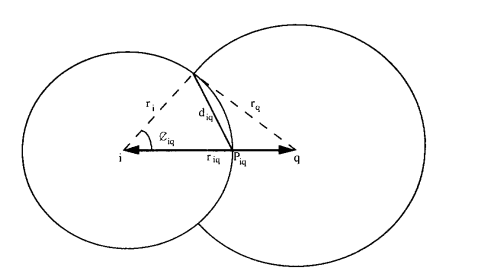
\includegraphics[width=3in]{mask}}
All points on $a_i$ within $d_i$ of the $P_{iq}$ are buried, and those bits in $m_{iq}$ are set to zero, with the rest set to 1. This string can be AND'ed with $b_i$ to produce a new $b_i$. This can be done for all spheres that intersect $a_i$ for each sphere in turn. The key insight that cuts down on the $nkl$ calculations is the fact that the $m_{iq}$ can be stored and retrieved later if the same string is ever needed. This is very likely to occur, because the $d_{iq}$ can be made independent of $r_i$ by removing the factor. Then $d_{iq}=\sqrt{2(1-\cos\theta_{iq})}$. Now we can calculate $m_{iq}$ for the range of $d_{iq}$ from 0-2.
\subsection{Richmond's Algorithm and the Gauss-Bonnet Theorem}
In a previous paper written by Richmond (1984), a different strategy is used to find the solvent exposed surface area of the atoms. He still represents the atoms as spheres with definite radius with centers at the atomic coordinates, but instead of using the Alpha Shapes, he made use of the Gauss-Bonnet theorem, a fundamental theorem in differential geometry which connects the topological properties of a manifold (specifically its Euler Characteristic) with its geometric properties (its curvature). A standard statement of the theorem is 
\begin{equation}
\int_M KdA + \int_{\partial M} k_g ds = 2\pi\chi(M)
\end{equation}
Here $\chi$ is the Euler Characteristic of $M$, and $K$ and $k_g$ are the Gaussian and geodesic curvatures of the manifold and the boundary respectively. For polygons, $\chi=V-E+F=1$. 

The SASA of an atom with radius $\varrho_i$ lies on a sphere where $K=\frac{1}{\varrho_i^2}$. We can divide this SASA into many polygons bounded by the circles of intersection with neighboring spheres (See Figure). If $M$ is one particular region of that SASA, we can write 
\begin{align}\nonumber
&\frac{1}{\varrho_i^2}\int_M dA + \int_{\partial M} k_g ds= 2\pi \\
&\implies A=\varrho_i^2\left(2\pi-\int_{\partial M} k_g ds\right)
\end{align}

\begin{figure}[h!]
\caption{Two Intersecting Spheres}
\centerline{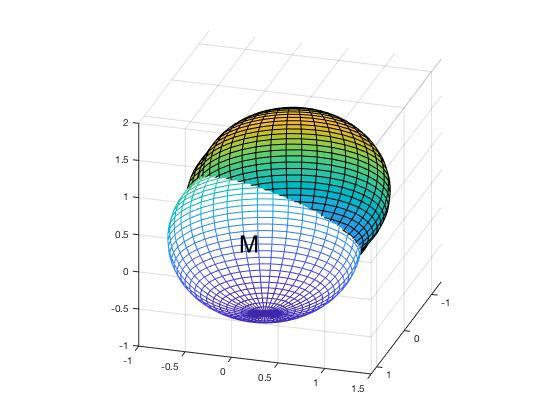
\includegraphics[width=3in]{spheres}}
\end{figure}
Thus if we know $k_g$ (the geodesic curvature) of the boundary of $M$ at all points, we can compute $A$. If $\partial M$ is piecewise smooth, then $\int_{\partial M} k_g ds$ is the sum of the integrals along the components of the boundary plus the sum of the angles by which the elements of the boundary turn at the corners. For the simple example of a geodesic triangle on a sphere of radius $\rho$, $\int_\gamma k_g ds=0$ where $\gamma$ is a piece of $\partial M$. Thus $\int_{\partial M} k_g ds=0+\sum (\pi-\alpha_i)$, where $\alpha_i$ are the interior angles of the triangle. Plugging this into $(5)$ gives $A=\rho^2(-\pi+\sum\alpha_i)$. This is the well known Girard's Theorem. 

In our case, the boundaries of $M$ won't be piecewise geodesic, and thus calculating $\int_{\partial M} k_g ds$ will require knowledge of the circles of intersection between the spheres. With that data calculating $k_g$ simply requires some vector calculus$^1$.
We can calculate the SASA of the entire protein this way, by adding up the contributions of the individual regions $M$ across all atoms.

\section{The Power Diagram Model}
\subsection{Power Diagrams}

Our protein can be represented as a set of atom centers $S$ in $\R^3$ with their corresponding balls of various radii. One aspect of the model is computing the power diagram of this protein. The power diagram is a generalized Voronoi diagram, where instead of the normal Euclidean metric, the definition for distance between an atom with center $z_i$ and radius $\varrho_i$ and a point $x$ is $\pi_i(x)=\|x-z_i\|^2-\varrho^2$. This becomes the default Voronoi diagram of $S$ if all the radii are equal. After this power diagram is generated we can associate each atom $S_i$ with its corresponding power cell $P_i$ defined by
\begin{equation*}
P_i=\{x\in\R^3\mid\pi_i(x)\leq\pi_j(x),\forall j\}
\end{equation*}
Each $P_i$ is convex, and together they cover all $\R^3$ without overlap. The dual of this power diagram is a weighted Delaunay Triangulation of $S$ into a set of simplices. We can compute the surface area of these balls using Delaunay triangulation, which will help us in the later sections. There are additional rules for constructing Delaunay triangles, but for the purposes of this paper, it is only necessary to know what the vertices of each triangle represent. 

\begin{comment}
To draw the Delaunay triangles, the centers of the balls are taken to be the vertices of the triangles. If any two circles have adjacent power cells, an edge will be drawn between them. Every three power cells with a common edge will make up a triangle and a tetrahedron will comprise four power shells with a common vertex.
\end{comment}

\begin{comment}
Before launching into how the authors modeled and derived area equations for computational molecular modeling, we should discuss the concept behind $\alpha$-shapes.  $\alpha$-shapes are the foundation of this model, and knowing what they are will help us better understand the derivations presented in the further sections. Hence imagine a set of points in $\R^3$ and we want to describe the 'shape' of these points. One solution is the convex hull of these points, which has been quite well studied. However $\alpha$-shapes are hulls that still include all points, but so so in finer detail than the standard convex hull. Constructing an $\alpha$-shape can be thought of via the following analogy from Fischer$^2$.

Imagine a mass of $M\&M$ ice cream in $\R^3$, with a point set $S$ suspended in it like a set of $M\&M$'s. Using a spherical ice cream scoop with radius $\alpha$, we start removing all parts of ice cream we can reach without removing the $M\&M$'s. This includes internal scoops that might not be reachable from the outside. The remaining mass will be an $\alpha$-shape of the set of $M\&M$'s. By varying $\alpha$ from 0 to $\infty$, the corresponding $\alpha$-shape goes from $S$ itself to the standard convex hull of $S$. Convex hulls and $\alpha$-shapes are important because the Delaunay Triangulation of a set in $\R^n$ can be viewed as the projection of the corresponding convex hull in $\R^{n+1}.^3$ Thus we can find the Delaunay Triangulation of the set of atom centers by calculating the convex hull. This computation is also quite fast.
\end{comment}

\begin{comment}
Alpha-Shapes are a subset of Delaunay Triangulation, a method that separates a surface into a series of triangles in order to make it easier to identify properties of an object. Alpha-Shapes are more generally known as being comprised of many such triangles, or simplexes. Using Alpha-Shapes makes studying three-dimensional balls in space (or molecules) much easier. It provides a way to run computations faster, especially when given large amounts of data. Molecules like proteins are often made with hundreds or thousands of three-dimensional balls, so using the Alpha-Shapes method is very practical for these purposes. 

The dual of this Delaunay Triangulation is called the Voronoi Diagram of the atom centers.
The term “Voronoi diagram” is often used to classify the partition of a plane. Each partition is referred to as a “Voronoi cell” (Edelsbrunner). In his paper, Edelsbrunner uses the term “Voronoi cells” to describe each d-ball in $R^3$ (or 3-ball), which has a center z with some point x. The authors describe the atoms as being surrounded by a solvent sphere, which will be elaborated in the next section. Briefly, this model is represented by several terms. First, the power distance of x from b is
\\$\pi_i(x) = ||x-z_i||^2 - (\varrho)^2 $
\\The power distance is the distance from some point in the ball to the solvent shell. The power cell is what minimizes this distance between the point and the solvent shell.
\\$P_i = {x \epsilon \R^3 | \pi_i(x) <= \pi_j(x) \forall j}$
\\All of these spheres, or the alpha-shape, are what’s known as a power diagram. 
\end{comment}

\subsection{Application to Protein Structures}
\begin{comment}
To represent the entire state of the protein (with $n$ atoms) we use the $m=3n$ dimensional  vector \textbf{z}, where consider a set of balls $B_i$ defined by a center $z_i$ and a fixed radius $\varrho_i$ to be in some state \textbf{z} in $\R^{3n}$. Each ball $B_i$ is surrounded by a sphere $S_i$ in this state. It is stated that if any space in $\R^m$ can be approximated by a linear space ($\R$), it is possible to find its derivative. By considering this differentiable map f, which takes the object from $\R^m$ to$\R$, they use this reasoning to say that the derivative of this map is linear. Thus, the authors show that it can be represented by vectors known as \textbf{t} and \textbf{u}, both of which are in $\R^m$, where \textbf{t} is a some variable vector and \textbf{u} is a gradient vector that shows how it changes with \textbf{t}. So the derivative of f will map each \textbf{z} to its gradient, or direction vector. The paper considers a space of $\R^3$ to better represent atoms. It states that m = 3n (so the balls are in $\R^{3n}$), and i can be no less than n-1. So, for some \textbf{z} or $B_i$, the center of $B_i$($z_i$) is stated as $(textbf{z}_{3i+1},textbf{z}_{3i+2},textbf{z}_{3i+3})$. The radius of $B_i$ is noted to be $\varrho_i$.
\end{comment}

Consider a set of balls $B_i$ defined by a center $z_i$ and a fixed radius $\varrho_i$ to be our protein. To represent the entire state of the protein (with $n$ atoms) we use the $m=3n$ dimensional  vector $\textbf{z}\in\R^{3n}$ where $\lbrack{\bf z}_{3i+1}, {\bf z}_{3i+2}, {\bf z}_{3i+3}\rbrack^T=z_i$. Now we can define the weighted and unweighted surface areas $W,A:\R^{3m}\rightarrow\R$ as real multivariate functions from the state of the protein to a single value (the solvent exposed surface area). The weighted area will be described below. Here we will describe the gradients of these maps, written as $DW_{\bf z}$ and $DA_{\bf z}$ which would allow us to calculate SASA's for protein structures and approximate how the SASA changes as the atomic coordinates move. These derivatives map each point in $\R^m$ to a corresponding gradient vector that we call $u$.

\begin{figure}[h!]
\caption{$B_1$ where $n = 2$ is bound by a solvent sphere. The radius of the solvent is the distance between the edge of the ball and the sphere.}
\centerline{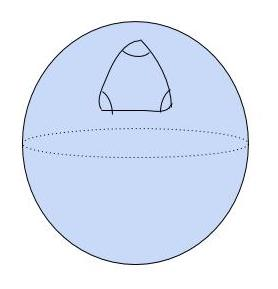
\includegraphics[width=3in]{Figure3}}
\end{figure}

You can imagine that given a collection of atoms, there will be many balls in one space with their spheres overlapping (Figure 2).The area derivative equations are describes for groups of two or three overlapping spheres, which can be applied to larger systems. Using the Power Method method described above, we can use Delaunay Triangulations to assist with their calculations.

\begin{figure}[h!]
\caption{Three balls in space bounded by three different spheres. Their centers are used for Delaunay Triangulation.}
\centerline{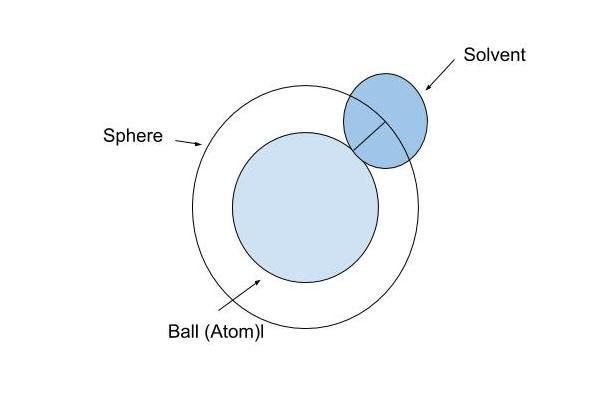
\includegraphics[width=3in]{Figure8}}
\end{figure}


%The authors make use of a power diagram for their model, which is another name for the structure of spheres shown in Figure 2. Just like we mentioned previously, the power diagram consists of power cells. [Repetitive]

\begin{figure}[h!]
\caption{A power diagram comprised of power cells (left) and its Delaunay Triangulation (right).$\lbrack1\rbrack$}
\centerline{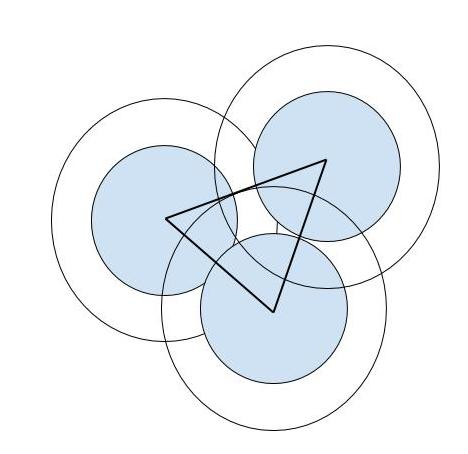
\includegraphics[width=3in]{Figure2}}
\end{figure}


In order to get to the derivation, we must define some additional terms. After constructing Delaunay Triangles from a set of molecules, they note two important terms , "star" and "link", that are useful for defining area equations. Each Delaunay triangle is a simplex, where simplex is the higher dimensional analogue of a triangle or tetrahedron. They define K as a dual complex, or subcomplex of the alpha shape.

\begin{figure}[h!]
\caption{The dual complex (K) of the Delaunay Triangulation only includes those power cells that non-empty intersection.$\lbrack1\rbrack$}
\centerline{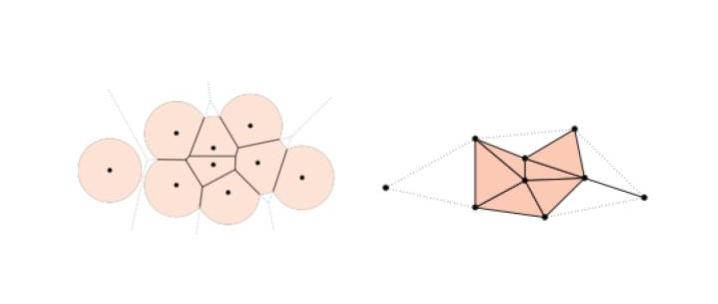
\includegraphics[width=3in]{Figure4}}
\end{figure}

K is made up of multiple simplices. The “star” of K would then just be a set of triangles who share a vertex and outside boundary. They also define the “link” of K to be all of the vertices and edges in the star.

\begin{figure}[h!]
\caption{The star of K and link of the star are shown.$\lbrack1\rbrack$}
\centerline{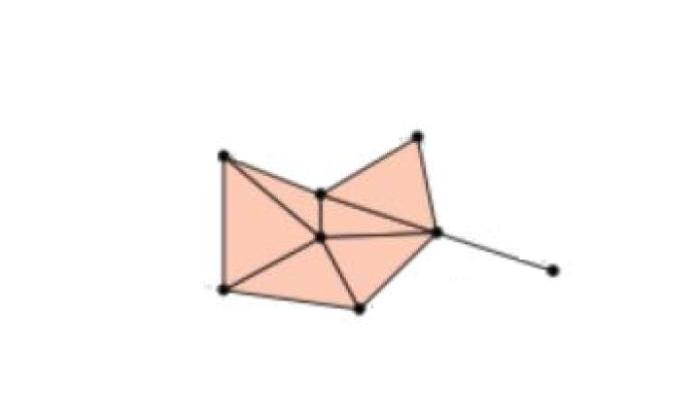
\includegraphics[width=3in]{Figure9}}
\end{figure}

Knowing how the star and link of a subcomplex K are defined will help find the solvent-exposed surface area.
The space-filling diagram, or collection of spheres, is represented by $F$. $F_i$, for instance, consists of all the points in $B_i$. $\sigma$ represents the fraction of a sphere on a boundary of $F$. We care about the boundary of $F$ because that contributes to the exposed surface area, unlike the intersecting portion of the sphere. So for two intersecting balls, our equation comes out to:

\begin{equation*}
\sigma_{ij} = \frac{length(P_i \cap P_j \cap bd F}{length(S_{ij})}
\end{equation*}

This means that for two intersecting balls i and j,$\sigma_{ij}$ will be the fraction of the exposed (hence bd F) surface that's on the power cells of each of the balls. 
Using the dual complex, we can specify the following equation for $\sigma_{ij}$ in terms of two intersecting circles, which will become useful later.
\begin{equation}
\sigma_{ij} = \frac{1 - (\sum_{k}length(S^k_{ij}) - \sum_{k,l} length(S_{ij}^2 \cap S^l_{ij}))}{2\pi\varrho_{ij}}
\end{equation}

They derive this equation by looking at Edelsbrunner's (1995) paper. They consider two spheres $S_i$ and $S_j$, which intersect at a circle. $S^k_{ij}$ and $S^l_{ij}$ are two other spheres that minimize the power distance to the circle of intersection. Subtracting the term on the right from 1 gives the fraction of exposed surface area.

$\sigma$ is related to the area of the ball, which for a ball with radius $\varrho$ is $4pi\varrho^2$. However, we are only concerned with exposed area. This means that we need to multiply by $\sigma$, the fraction of the ball that’s exposed, in order to only get the solvent-exposed surface area. We can also define a weighted area, which only differs by the area equation by the factor of some parameter $\alpha$, which represents some constant atomic solvation parameters that were predefined by Eisenberg and McLachlan(1986). So for just one ball $B_i$:
\begin{align*}
&A = 4\pi\sum\varrho_i^2\sigma_i \\
&W = 4\pi\sum\alpha_i\varrho_i^2\sigma_i
\end{align*}

Another term, $\beta_{ijk}$, is also used, which is useful when considering the case of three intersecting balls. When three spheres intersect at two points, there is a line segment passing through them that is represented as $B_{ijk}$. Just like for $\sigma_{ij},\beta_{ijk}$ represents the fraction of points that belong to the edge of F, the space-filling diagram and 
\begin{equation}
\beta_{ijk} = \frac{length(P_i \cap P_j \cap P_k \cap bd F)}{length(B_{ijk})}
\end{equation}

The equation above shows that $\beta_{ijk}$ represents the fraction of the exposed points that are on the intersection of the three spheres. A similar expression to $\sigma_{ij}$ is derived for $\beta_{ijk}$, using $B^l_{ijk}$, the portion of the line segment on a fourth sphere (l). By subtracting the right term from 1, the solvent exposed area for three intersecting spheres is found.

We can think of the sphere as representing how much of the solvent can interact with the atom. The state z of each ball defines a center and a radius. This paper considers that the weighted (E) and unweighted (A) areas are transformations from the space containing \textbf{z} $(R^3n)$ to R. Their derivatives at a particular \textbf{z} are linear maps. In other words, the areas are represented by the map f and their derivatives the derivative of f at \textbf{z}.
\subsection{Direction Preserving Motion} 
In this type of motion, it is assumed that two spheres $S_i$ and $S_j$ bounded with a non-empty intersection are moving on the line passing through their centers.
Let’s again consider F to be the space-filling diagram of each sphere. $F_i$ is then the union of $B_i$ and  $F_j$ is the union of $B_j$. We can assume the spheres of both atoms intersect each other (Figure 3) So, we can say that F contains the points that are the union of $B_i$ and $B_j$, or all the points in balls $i$ and $j$. So we are assuming the atoms are intersecting each other.

\begin{figure}[h!]
\caption{Two intersecting spheres $S_i$ and $S_j.\lbrack1\rbrack$}
\centerline{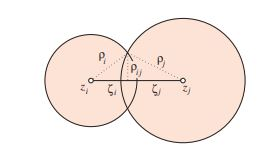
\includegraphics[width=3in]{Figure6}}
\end{figure}


Let's show how $\zeta_i^2 - \zeta_j^2 = \varrho_i^2-\varrho_j^2$ and then show how $(\zeta_i)^2 (\zeta_j)^2 $ simplifies to $\zeta_{ij}*(\zeta_i - \zeta_j)$. First assume the following equations for the spheres:

\begin{align*}
&x^2 + y^2 +(z-z_i)^2 = \zeta_i^2 \\
&x^2 + y^2 +(z-z_j)^2 = \zeta_j^2 \\
&\implies \zeta_i^2-\zeta_j^2 =(z-z_i)^2-(z-z_j)^2=-2z_i +2z_j +z_i^2 - z_j^2\\
\end{align*}
Using this logic, we can find the same equation holds true if we consider the atoms (balls), as they have the same centers as the spheres. So:
\begin{align*}
&-2z_i +2z_j +z_i^2 - z_j^2 = \varrho_i^2-\varrho_j^2 \\
&\zeta_i^2-\zeta_j^2 = \varrho_i^2-\varrho_j^2\\
&\text{We can factor out $\zeta_i^2-\zeta_j^2$ to get:} \\
&\zeta_i^2-\zeta_j^2 =(\zeta_i-\zeta_j)(\zeta_i+\zeta_j) = \zeta_{ij}(\zeta_i-\zeta_j) \\
&\text{Now we can find what $\zeta_i$ and $\zeta_j$ really are} \\
&\varrho_i^2 - \varrho_j^2  = \zeta_{ij}(\zeta_i-\zeta_j) \\
&(\varrho_i^2 - \varrho_j^2)/\zeta_{ij} + \zeta_j = \zeta_i \\
&\text{We know that $\zeta_j = \zeta_{ij} - \zeta_i$, so just substitute this expression in:} \\
&\zeta_i = \frac{1}{2}\left(\zeta_{ij}+\frac{\varrho_i^2-\varrho_j^2}{\zeta_{ij}}\right) \\
&\text{A similar statement can be made for $\zeta_j$, following the steps we carried out above:} \\
&\zeta_j = \frac{1}{2}\left(\zeta_{ij}+\frac{\varrho_j^2-\varrho_i^2}{\zeta_{ij}}\right)
\end{align*}

Now we can find the area of both spheres. We know that $A = 4\pi r^2$. For two spheres $A = A_i + A_j$. Recall the area equation stated in the model. For two balls we can say: $A = 4\pi\varrho^2\sum{\sigma_i} + 4\pi\varrho^2\sum{\sigma_j}$. After plugging in $\sigma$ and simplifying the area equation:
\begin{align*}
&4\pi\varrho^2\frac{\varrho_i + \zeta_i}{2\varrho_i} + 4\pi\varrho_j^2\frac{\varrho_j + \zeta_j}{2\varrho_j} \\
&\text{After a few algebraic simplifications:} \\
&2\pi\varrho_i^2 +2\pi\varrho_j^2 +\pi\varrho_i\left(\zeta_{ij} + \frac{\varrho_i^2 - \varrho_j^2}{\zeta_{ij}}\right)+\pi\varrho_j\left(\zeta_{ij} + \frac{\varrho_j^2 - \varrho_i^2}{\zeta_{ij}}\right) \\
&A  = 2\pi*(\varrho_i^2 + \varrho_j^2) + \pi(\varrho_i+\varrho_j)\left[\zeta_{ij}+\frac{(\varrho_i-\varrho_j)^2}{\zeta_{ij}}\right] \\
&\text{Then we find the derivative of the area with respect to $\zeta_{ij}$} \\
&\frac{dA}{d\zeta_{ij}} = \pi(\varrho_i+\varrho_j)\left[1-\frac{(\varrho_i - \varrho_j)^2}{\zeta_{ij}^2}\right] \\
&\text{This is term they get after some simplification.}
\end{align*}

\subsection{Distance Preserving Motion}
In distance preserving motion, one sphere rotates about another.
Imagine three spheres interesting at two points. This time, $F$ is going to include all the points contained in all three balls. If the spheres intersect at two points then one sphere contains both of them. Next, consider the caps of the spheres i and k when finding the exposed surface area ($C_{ij}$ and $C_{kj}$). The caps intersect and we can find the parameters for these similar to how we found the formulas for the direction preserving motion. This model says that as you move the two caps apart, keeping their centers in the same position, you will gain an area equal to that of a spherical rectangle.
\begin{figure}[h!]
\caption{Three intersecting spheres at two points: $S_i$, $S_k$ and $S_j.\lbrack1\rbrack$}
\centerline{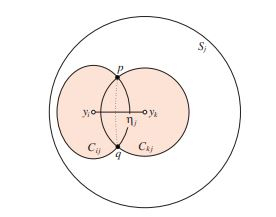
\includegraphics[width=3in]{Figure7}}
\end{figure}

Using this spherical rectangle shape, the we find the area to be the difference between the center of the circles divided by the circumference of the larger ball (which is in this case) times the area of the slice of $S_j$ between $p$ and $q$. The area derivative of this larger ball becomes: $\frac{dA_j}{d\eta_j} = 2\varrho_{ijk}$

\subsection{Combining the Area Equations} 
After we’ve looked at how to find the area derivatives, we can see how they’re able to come together. As was mentioned before, because the derivatives are linear, they can be separated into a sum of their components. For the case of the direction-preserving motion, $u_{ij} = \frac{z_i - z_j}{\zeta_{ij}}$ , showing that the gradient is dependent on the distance between the two centers of $S_i$ and $S_j$. The gradient vector for the distance preserving motion is dependent on the component of the intersection to two of the spheres ($u_{ik}$) that is normal to the component of intersection between the other two spheres ($u_{ij}$). This makes $u_{ijk} = \frac{u_{ik} - <u_{ik},u_{ij}> \cdot u_{ij}}{\|(u_{ik} - <u_{ik},u_{ij}>) \cdot u_{ij}\|}$

Based on the above derivation above, we can state the unweighted and weighted area derivative theorems . Remember that we said each state 	\textbf{z} was in $\R^3n$, and each \textbf{z} represents set of balls $B_i$ so that $0<=i<=n-1$. So the center of $B_i$ is represented by $z_i$, which is equal to $\lbrack\textbf{z}_{3i+1},\textbf{z}_{3i+2},\textbf{z}_{3i+3}\rbrack$. Looking at the area derivative theorem, the derivative of the area at some \textbf{z} to be $DA_z(\textbf{t}) = <\textbf{a},\textbf{t}>$, where \textbf{a} is a gradient vector like \textbf{u} and 	\textbf{t} is the variable vector mentioned above. They state that for the unweighted area derivative, 
\begin{equation}
\textbf{a} = \sum_j \sigma_{ij}\cdot a_{ij}+ \sum_j \sum_k \beta_{ijk}\cdot a_{ijk}
\end{equation}

The first sum shows the contribution of the direction preserving motion while the second sum shows the contribution of the distance preserving motion. We can see for the first sum that we are summing over all of the points along the boundary when considering the intersection of two spheres $S_i$ and $S_j$, and the second sum considers the sum of points along the intersection for three intersecting spheres. Also for $a_{ij}$ and $a_{ijk}$:
\begin{align*}
&a_{ij} = \pi*(\varrho_i+\varrho_j)*\left[1 - \frac{(\varrho_i - \varrho_j)^2}{\zeta_{ij}^2}\right]\cdot u_{ij} \\
&a_{ijk} = 2\varrho_{ijk}\frac{\varrho_i - \varrho_j}{\zeta_{ij}} \cdot u_{ij}
\end{align*}

The weighted area derivative theorem, defined as $DE_z(\textbf{t}) = <\textbf{e},\textbf{t}>$ is defined similarly to the area derivative theorem, but multiplied by the solvent parameter $\alpha$ i.e

\begin{align*}
&\textbf{e} = \sum_j \sigma_{ij}\cdot e_{ij}+ \sum_j \sum_k \beta_{ijk} \cdot e_{ijk} \\
&e_{ij} = \pi\left((\alpha_i\varrho_i +\alpha_j\varrho_j) - \frac{(\alpha_i\varrho_i  - \alpha_j \varrho_j)(\varrho_i^2 - \varrho_j^2)}{\zeta_{ij}^2}\right)\cdot u_{ij} \\
&a_{ijk} = 2\varrho_{ijk}\frac{\alpha_i\varrho_i - \alpha_j\varrho_j}{\zeta_{ij}}\cdot u_{ij}
\end{align*}

Above, we described $\textbf{a}$ and $\textbf{e}$. Using these, we can the clearly state the area derivative equations. For the unweighted area derivative equation, the direction preserving component is the the fraction of the solvent-exposed surface times the derivative of the area: $\sigma_{ij}<a_{ij},t_i>$ and the distance preserving component is the same: $\beta_{ijk}<a_{ijk},t_i>$. We know that the unweighted area derivative is the sum of these two components:
\begin{equation}
DA_z(\textbf{t}) = \sum_{i=0}^{n-1}\sum_{j!=i}\left(\sigma_{ij}<a_{ij},t_i> + \sum_{k!=i,j} \beta_{ijk}<a_{ijk},t_i>\right)
\end{equation}
Just like before, the weighted area derivative is basically the same as the unweighted derivative: 
\begin{equation}
DE_z(\textbf{t}) = \sum_{i=0}^{n-1}\sum_{j!=i}\left(\sigma_{ij}<e_{ij},t_i> + \sum_{k!=i,j} \beta_{ijk}<e_{ijk},t_i>\right)
\end{equation}

\subsection{Model Assumptions}
As explained above, one of the biggest assumptions made is by representing each atom as a ball. This ball is surrounded by a sphere whose distance from the edge of the ball represents the radius of a solvent sphere (Figure 1). A solvent refers to a liquid the molecule is suspended in, usually water. Another assumption to point out is that water is being represented as a sphere (continuously) rather than a collection of atoms. 


\section{Application of ALPHAMOL to Molecular Modeling}
To test the time cost of \textsc{alphamol} (the computational implement of the method described in $\S3$) we took 250 PDB structures from the RCSB database (listed in the supplemental) and calculated the number of polar atoms buried in the structure that are not making hydrogen bonds. This calculation indirectly uses a SASA calculator to determine if atoms close to the surface are truly buried. If they have any SASA that is nonzero, the atom is assumed to be making a hydrogen bond with the implicit solvent. We compared the time taken to complete the buried unsatisfied polars calculation for the \textsc{alphamol} and Shrake-Rupley SASA calculators. We found that \textsc{alphamol} is slower, but it is more accurate.


\section{Glossary}
\begin{align*}
&\varrho_i:&\text{The radius of ball i} \\
&z_i:&\text{The center of a ball i} \\
&{\bf z}:&\text{The $3n$ dimensional vector representing the state of all $z_i$} \\
&\zeta_{ij}:&\text{The signed distance between centers of two intersecting spheres} \\
&\sigma_{ij}:&\text{The fraction of solvent-exposed surface for two intersecting spheres $S_i,S_j$} \\
&\beta_{ijk}:&\text{The fraction of solvent-exposed surface for three intersecting spheres $S_i,S_j, S_k$} \\
&\alpha:&\text{An atomic solvation parameter} \\
&F:&\text{The space filling diagram} \\
&\pi_i(x):&\text{The power distance of a random point x from $S_i$} \\
&P_i:&\text{The set of points closer (by power distance) to $S_i$ than any other sphere} \\
&K:&\text{The dual complex of Delaunay Triangulation. Consists of all power cells with non-empty intersection} \\
&DA_{\bf z}({\bf t}):&\text{The unweighted area derivative at \textbf{t}} \\
&DW_{\bf z}({\bf t}):&\text{The weighted area derivative at \textbf{t}} \\
\end{align*}


\listoffigures

\begin{thebibliography}{9}

\bibitem{DeCoste}
DeCoste, Donald J., Zumdahl, Steven S. General Chemistry 142 University of Washington 7th Edition, Boston, Cengage Learning, 2015.

\bibitem{Edelsbrunner} 
Edelsbrunner, H. The Union of Balls and Its Dual Shape. Discrete \& Computational Geometry. 13 (1995), 415-440.

\bibitem{Fischer} 
Fischer, Kaspar. Introduction to Alpha Shapes. Stanford University, lecture notes, 2011.

\bibitem{Levitt} 
Bryant, R., Edelsbrunner, H., Koehl, P., Levitt, M. The Area Derivative of a Space-Filling Diagram. Discrete \& Computational Geometry. 32 (2004), 293-308.

\bibitem{Richmond}
Richmond, Timothy J. Solvent Accessible Surface Area and Excluded Volume in Proteins. J. Mol. Biol. 178 (1984), 63-89.

\bibitem{Rotskoff}
Rotskoff, Grant. The Gauss-Bonnet Theorem. University of Chicago REU, paper, 2010

\bibitem{Schnell}
Schnell, Christian. The Gauss-Bonnet Theorem. talk at Columbus, 2004.

\end{thebibliography}
\end{document}  